PyGromosTools is a software package that builds on the long history of GROMOS. After initial development phases of the package, its structure and associated usage patterns were established with long-term stability in mind. Consequently, the implementation of PyGromosTools was preceded by identification of several design objectives that are in line with state-of-the-art API development: \cite{Henning2009, Blanchette2008, Bloch2006}
%
\begin{itemize}
    \item An API is easy to learn and memorize such that solving problems with it comes naturally. 
    \item The usage of an API should result in code that is easy to read and maintain.
    \item A well-designed API is hard to misuse and easy to extend.
    \item An API is complete and simple. 
\end{itemize}
%
With these considerations in mind, the resulting API should enable fast, reproducible, and expandable simulation setup and execution of MD simulations. Additionally, the API should align with fundamental scientific principles to make data and code easily accessible, shareable, and reproducible. The importance of open and reliable data was already introduced and highlighted in Chapter \ref{ch:feens}.

\subsection{Coding Style}
PyGromosTools follows several coding styles. These are not enforced on the users but on the developers who would like to contribute to the API. 

\subsubsection{Code Visibility/Information Hiding}
Encapsulation is an essential concept in coding of larger projects. Only those layers of the software should be presented to a user, which are required to make the API still understandable or usable. Presenting the entire code basis of larger packages to end users may be overwhelming and hamper usage. Therefore, encapsulating code into functions and classes, or alternatively managing the accessibility of certain variables/functions is vital in code hiding.\cite{Leino2002, Ganney2020} Visible code should be easy to integrate and conveniently to use for writing more complex solutions.

In PyGromosTools, accessibility is managed with methods provided by Python. For example, private variables in the \textit{Gromos\_System} class are assigned with a prefix ``\_'' like the attribute \textit{\_gromosPP}. Note that this way of declaring a variable ``private'' still leaves it easily accessible, in contrast to other languages like C++. If a variable of function should never be used externally, name mangling is employed with the prefix ``\_~\_'' (like \textit{\_~\_ionDecorator}) as defined in the Python enhancement proposals (PEP) 8 (\url{https://www.python.org/dev/peps/pep-0008/}).
The second aspect of encapsulating code into functions and classes is achieved through modularization of the code. This concept allows quick construction of more complex structures, and therefore speeds up the development process and readability at the same time.\cite{Ganney2020}
One example in PyGromosTools is the file structure that is encoded by several classes, which represent the blocks, tables and fields of a GROMOS file (fields $\rightarrow$ blocks $\rightarrow$ file).

\subsubsection{Variables, Signatures, and Classes}
PyGromosTools in general follows the principle of using descriptive variables. Each name in the package should give a comprehensive description of the function of a given code section, and abbreviations are therefore discouraged. Following this style increases readability of the code, leads to improved understanding of code, and consequently reduces the number of errors. Along these lines, the second style decision for PyGromosTools is annotation of types for attributes in classes, function parameters, and function return types. This style is in accordance with PEP 526 (\url{https://www.python.org/dev/peps/pep-0526/}), PEP 484 (\url{https://www.python.org/dev/peps/pep-0484//}), and PEP 3107 (\url{https://www.python.org/dev/peps/pep-3107/}), in which a type annotation system was introduced to Python3. This decision was made due to the more complex data structures defined by PyGromosTools. Annotations provide guidance to users and developers on which data type is expected for a given function or attribute. The type annotations can be quickly accessed in the source code and also visualized in most modern IDEs or interactive Python sessions. A third style choice is the usage of keyword arguments for passing function parameters. Keyword argument passing was introduced with PEP 468 (\url{https://www.python.org/dev/peps/pep-0468/}). The underlying reason for the usage of this feature is the enhanced readability of the resulting code and an increased robustness to code refactoring of function signatures.

\subsubsection{Documentation and Continuous Integration}
In PyGromosTools, each function and module is expected to contain a docstring description. The chosen docstring style is following the numpydoc guidelines (\url{https://numpydoc.readthedocs.io/en/latest/format.html}) from the popular NumPy package.\cite{Vanderwalt2011} The docstring style is supported in various IDEs and automatically collected in the documentation generated by sphinx\cite{brandl2021}. As part of the documentation, PyGromosTools is accompanied by several Jupyter notebooks, which feature code examples applying the package in different use cases.\cite{Kluyver2016}
In addition to a comprehensive documentation, a continuous integration pipeline implements several steps that give insights into the code quality and correctness. The first step is performing unit tests that are implemented to check the core functionality of the PyGromosTools package. Every pull request to the main branch is automatically tested before merging, providing immediate information on potential bugs. Moreover, in the next step, a tool for test coverage was added such that developers can easily detect parts of the package for which no tests have been added yet. Nevertheless, all functionality added to the package must come with the corresponding unit tests. The final step is a syntax style guide that provides suggestions for improved readability and standardized code writing.

\subsubsection{Programming Paradigms}
Python3 is a multi-paradigm language that allows mixing of object-oriented programming (OOP)\cite{Kay1993} and functional programming paradigms. 
OOP enables the benefits of object inheritance and polymorphism.\cite{Ganney2020} These concepts are used extensively in PyGromosTools with state-driven contexts like file representations or the submission system classes. Especially the base class \textit{\_general\_gromos\_file} is a representative for the application of inheritance in the package. This class contains the fundamental read and write procedures that are identical for all GROMOS files and therefore only implemented once (see \url{https://github.com/rinikerlab/PyGromosTools/blob/main/pygromos/files/_basics/_general_gromos_file.py}).

Functional programming enables implementation of functions with Python's built-in map, apply, and zip operations, or using higher-order functional programming concepts like Python decorators.\cite{Ganney2020} As an example for the benefit of decorators, the principle of currying\cite{Curry1958} was realized for the GROMOS++ integration into the \textit{Gromos\_System}, such that dynamically generated functions update the attribute files of the \textit{Gromos\_System} automatically and those do not need to be provided to the function call (compare Figure \ref{fig: GROMOSSystemSimulationExample} versus Figure \ref{fig: GROMOSWrappers}, and function \textit{\_\_SystemConstructionUpdater} in \url{https://github.com/rinikerlab/PyGromosTools/blob/main/pygromos/files/\\gromos\_system/gromos\_system.py}).

\subsection{Code Structure}
PyGromosTools itself can be split into a high-level and a low-level layer. 
The low-level layer interfaces the operating system, the job queueing system, and the GROMOS wrappers. These functions are used in the high-level layer to build more complex structures like the \textbf{simulations} modules or the \textit{Gromos\_System}. 
%
In the following, we will discuss the implementation of different modules of PyGromosTools. In general, the package consists of four modules: \textbf{data}, \textbf{file}, \textbf{simulations}, and \textbf{analysis}.  


%The fundamental idea of files
\subsubsection{Files}
The \textbf{file} module is a collection of classes that represent the different GROMOS files in Python (Figure \ref{fig: FileModule}). The design of the module is based on considerations discussed in the context of OOP. It makes extensive use of inheritance and polymorphism to build up a class hierarchy consistent with the GROMOS file structure with minimal duplication of code.
In the GROMOS file structure, each file contains multiple blocks. These blocks in turn contain either a table of data or a sorted list of values. PyGromosTools represents this file structure such that the experienced behavior remains similar to the design of GROMOS. The structural basis is placed in the \textit{\_general\_gromos\_file} class, which contains the fundamental functionality encoded in the general file structure. Resulting functions are \textit{read\_file}, \textit{write}, and \textit{str}-operator overloading.
This generic file class encapsulates classes derived from \textit{\_generic\_gromos\_blocks}, which provide generic functions like read and write as well as operator overloading. 
The most basic data structure is used to store the content of generic blocks. This structure is for many blocks the \textit{\_generic\_field}, either a primitive or a Pandas data frame.
%
%Features
All these compartments generate specific classes for the different files used in the GROMOS environment. Features of these classes are: 
\begin{itemize}
    \item IO functionalities that not only allow writing of files but also writing obj states or converting files.
    \item Direct access of any type of GROMOS data in the objects enables a lean integration into Python3 scripts.
    \item Additional functionality that directly works on the file class includes calculating the root-mean-square deviation of MD trajectories or removing residues from coordinate files.
\end{itemize}

% generation of coordinates/atoms/molecules and topology generation of topology terms with correctness checking (is bond already present, etc. ) wrappers for simulation parameter blocks

\begin{figure}[h]
    \centering
    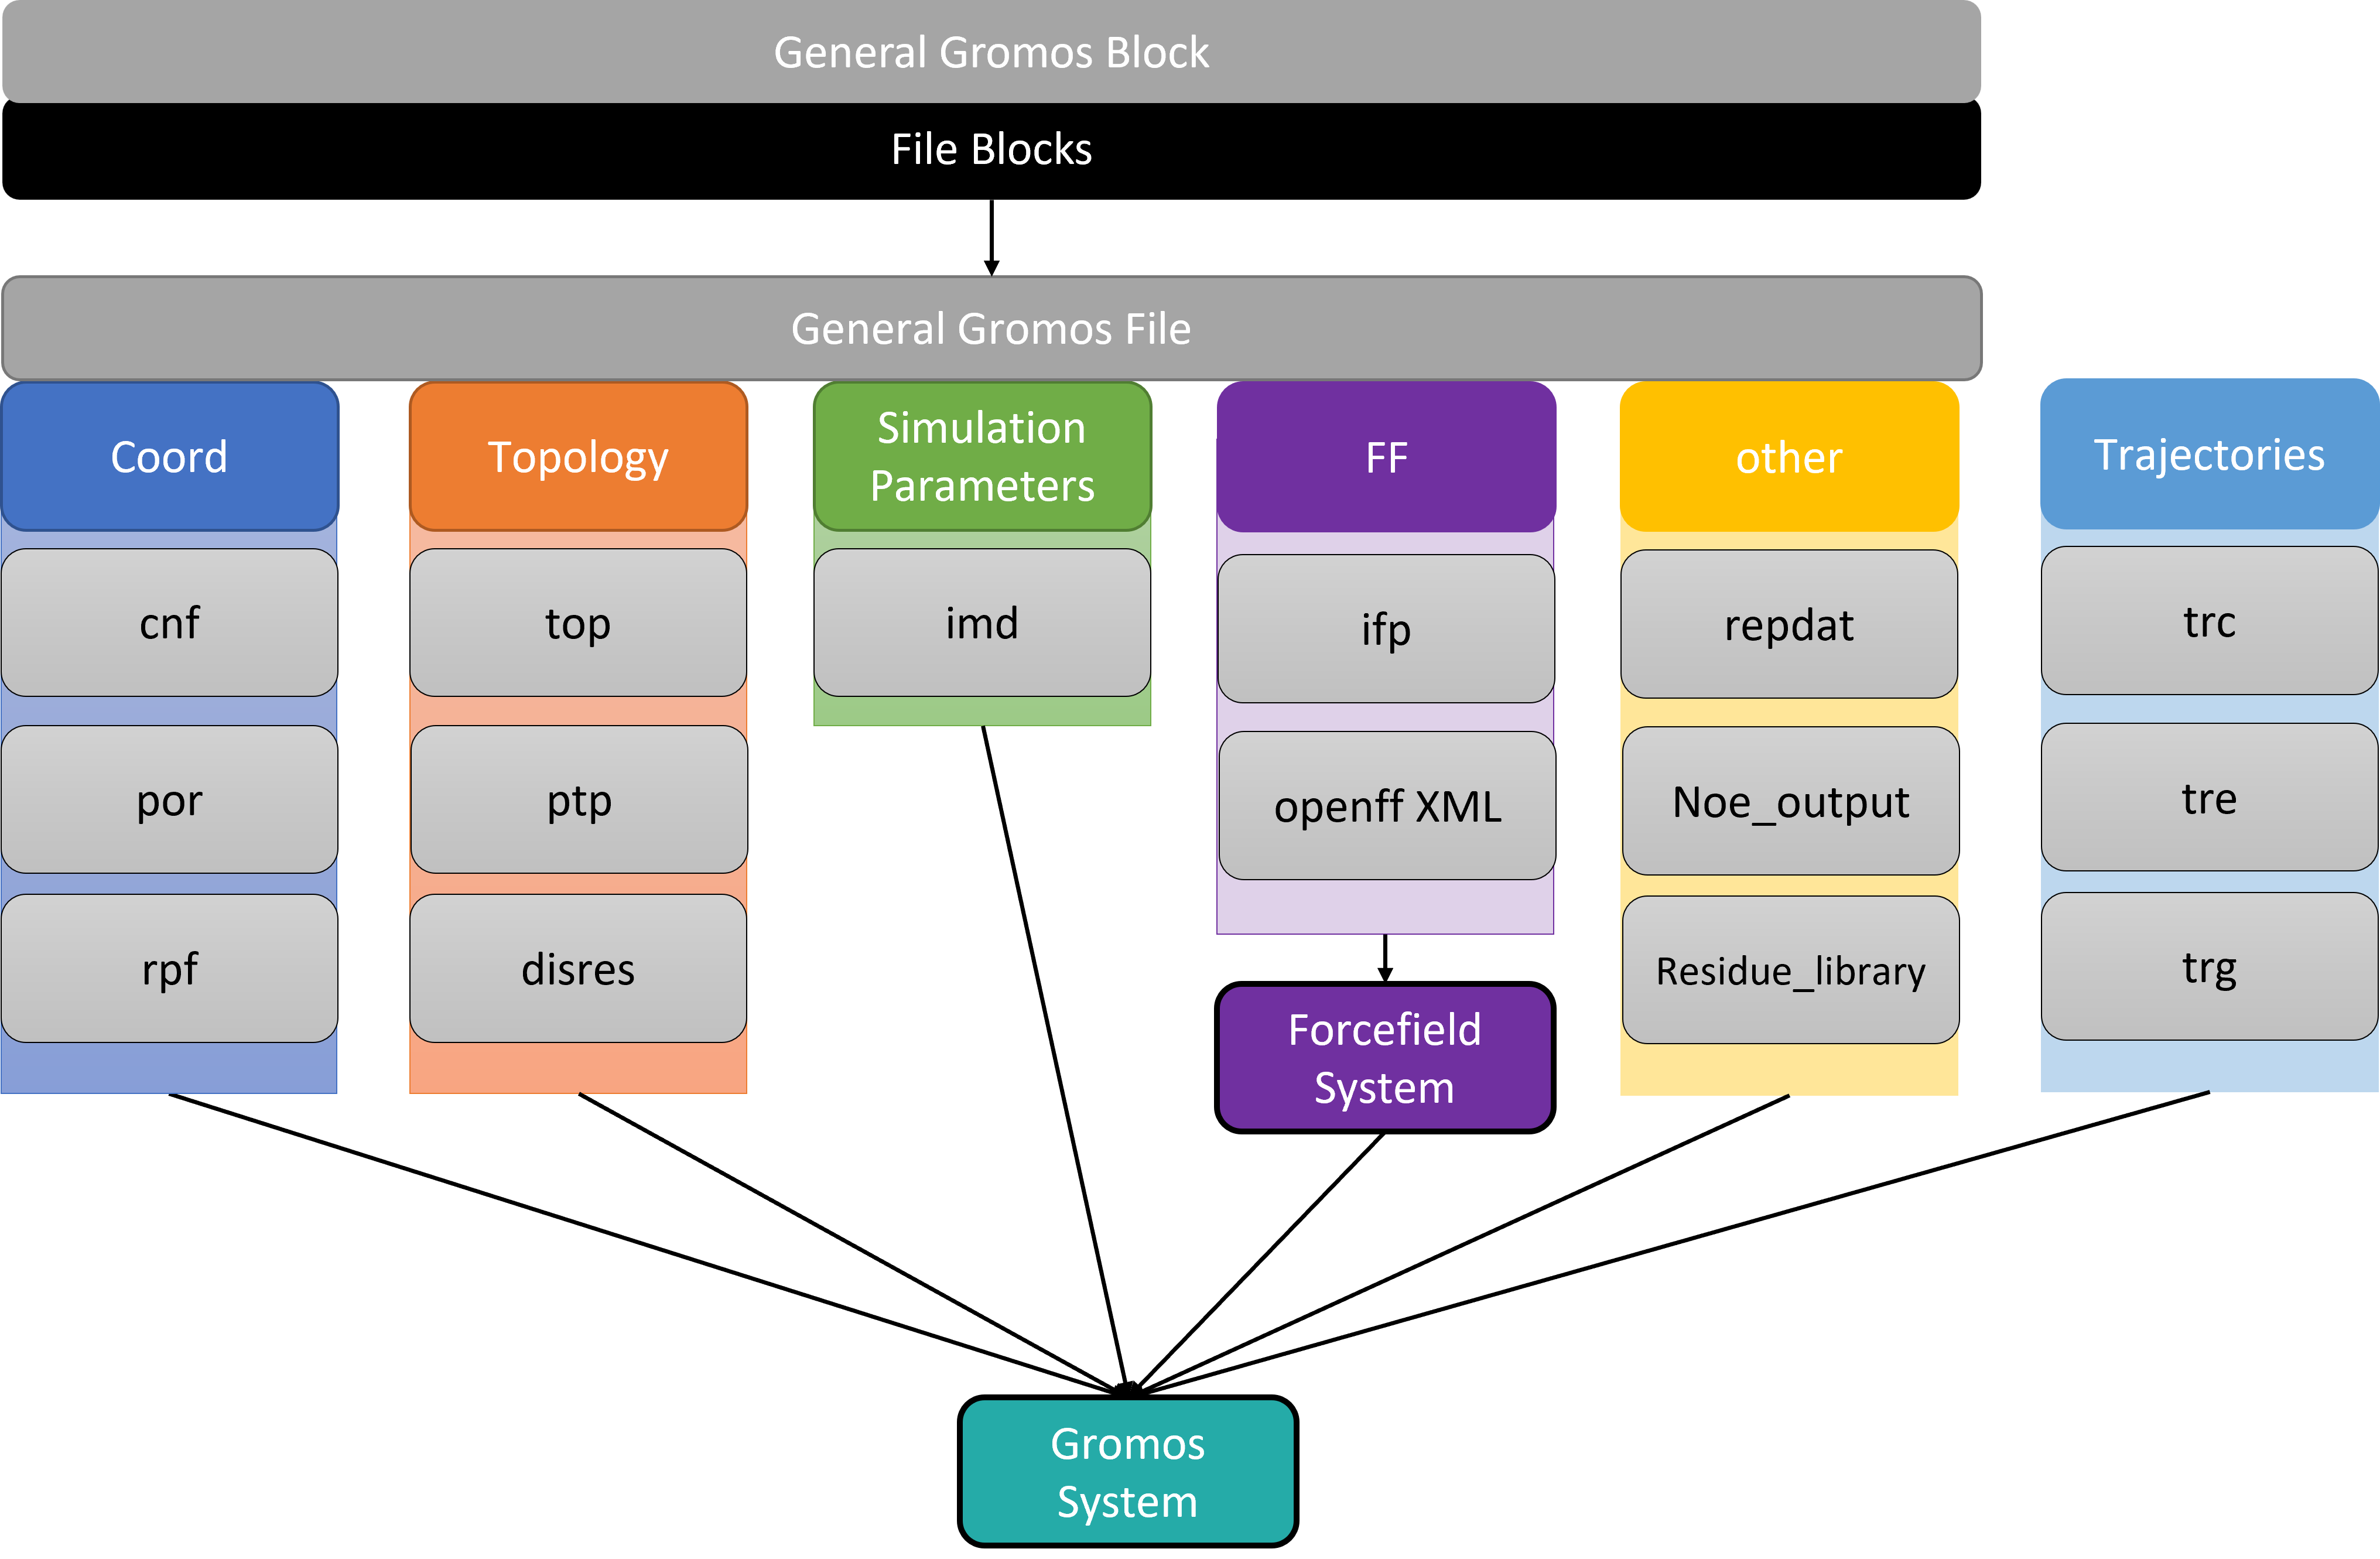
\includegraphics[width=\textwidth]{fig/implementation/Files.png} 
    \caption{PyGromosTools \textbf{file} module is implemented with an OOP structure based on the GROMOS file structure. The base classes are the \textit{\_generic\_GROMOS\_block} and the \textit{\_general\_GROMOS\_file}. From these base classes, all other GROMOS blocks and GROMOS files are derived (with the exception of trajectories) to provide a consistent user-experience.
    Only the implemented file classes are shown for clarity. The \textit{Gromos\_System} class collects all files and makes them easily accessible for simulation approaches or other functionality that requires multiple GROMOS files.
    }
    \label{fig: FileModule}
\end{figure}


%File Types
Most GROMOS files were implemented in PyGromosTools with an individual class derived from the base \textit{\_general\_gromos\_file} class, and sorted into the different categories according to their functionality (Figure \ref{fig: FileModule}). Due to the consequent class hierarchy, new blocks or files can be included very easily. 
The MD package involves many diverse types of files such as coordinate files, topology and simulation parameter files, coordinate and energy trajectory files, force-field files (FF), and others like replica-exchange outputs or NMR GROMOS++ program output files. The force-field class \textit{Forcefield\_System} represents a whole force field and contains the functionality to parametrize molecules.

With PyGromosTools, the MD trajectory files generated by GROMOS can be translated into a Pandas data frame for post-processing in Python. The data frame is stored in the compressed hf5 format \cite{Hf52020} to make it highly storage efficient and fast on I/O. Pandas data frames have the advantage that data is stored in NumPy arrays, which are internally implemented as C arrays. As a consequence, Pandas data frames are very memory efficient and basic mathematical operations on them (e.g., calculation of the mean, addition, etc.) are very fast, while these data frames still behave like Python objects.

%conc Outlook
In theory, PyGromosTools could also be used to introduce new file encodings without breaking legacy code. For example, the simulation parameters file could be translated into a JSON\cite{Pezoa2016} or XML\cite{Bray2008} data format, making file handling and readability easier by taking advantage of the key-value policy. In that regard, the Python ecosystem features a plethora of libraries that allow reading and writing these canonical file systems.


%%Gromos System
\paragraph{Gromos system}
All the different file formats implemented in PyGromosTools can be stored centralized in the \textit{Gromos\_System} class, which belongs to the high-level layer of PyGromosTools. This class is the central structure of PyGromosTools, from which systems are created or modified, simulated, and subsequently analyzed. The class can be used with a minimal set of files, i.e., a coordinate file (.cnf), topology file (.top), and a simulation parameter file (.imd), or just with a molecule SMILES or RDKit molecule to perform a complete automatic parametrization with a selected force field.
%
Two force fields can currently  be selected, the GROMOS Force Fields or the the open force field (OpenFF).\cite{Qiu2021} PyGromosTools provides tools to convert the OpenFF topology format to GROMOS format, perform sanity checks of the parameter files, or generate coordinate files from RDKit molecules. Additionally, the \textit{Gromos\_System} can adapt the simulation parameter file to use the correct functional forms required for the selected force field.
All functions can also be called ``manually''.

\subsubsection{Simulation Module}
The submodules of \textbf{simulations} can be arranged into three complexity layers. At the base are the \textbf{gromos} and \textbf{hpc-queuing} submodules. These submodules are used by the \textbf{simulation} module to provide simulation functionality to carry out energy minimizations or MD simulations. At the top is the \textbf{approaches} submodule, which uses the lower layers to facilitate complex simulation approaches like RE-EDS or for the calculation of the heat of vaporization. This layer structure enables fast adaptation and extension of functionality (Figure \ref{fig: SimulationModule}).
%
The submodule \textbf{gromos} contains the Python API to the GROMOS\cite{Schmid2012} and GROMOS++\cite{Eichenberger2011} binaries, providing quick access to their functionalities. The APIs of GROMOS and GROMOS++ are currently realized with bash wrappers, although a proper C++ Python integration would likely be beneficial to improve the communication between the layers. A \textbf{pyGROMOSPP} compartment has been added that contains efficient Python implementations of several programs available in GROMOS++. In general, we anticipate that the advantages of the Python language will lead to more GROMOS++ functionality being implemented directly into the Python layer. Note that the \textbf{gromos} submodule can be used isolated from all other modules.

%Simulation Approaches
\begin{figure}[h]
    \centering
    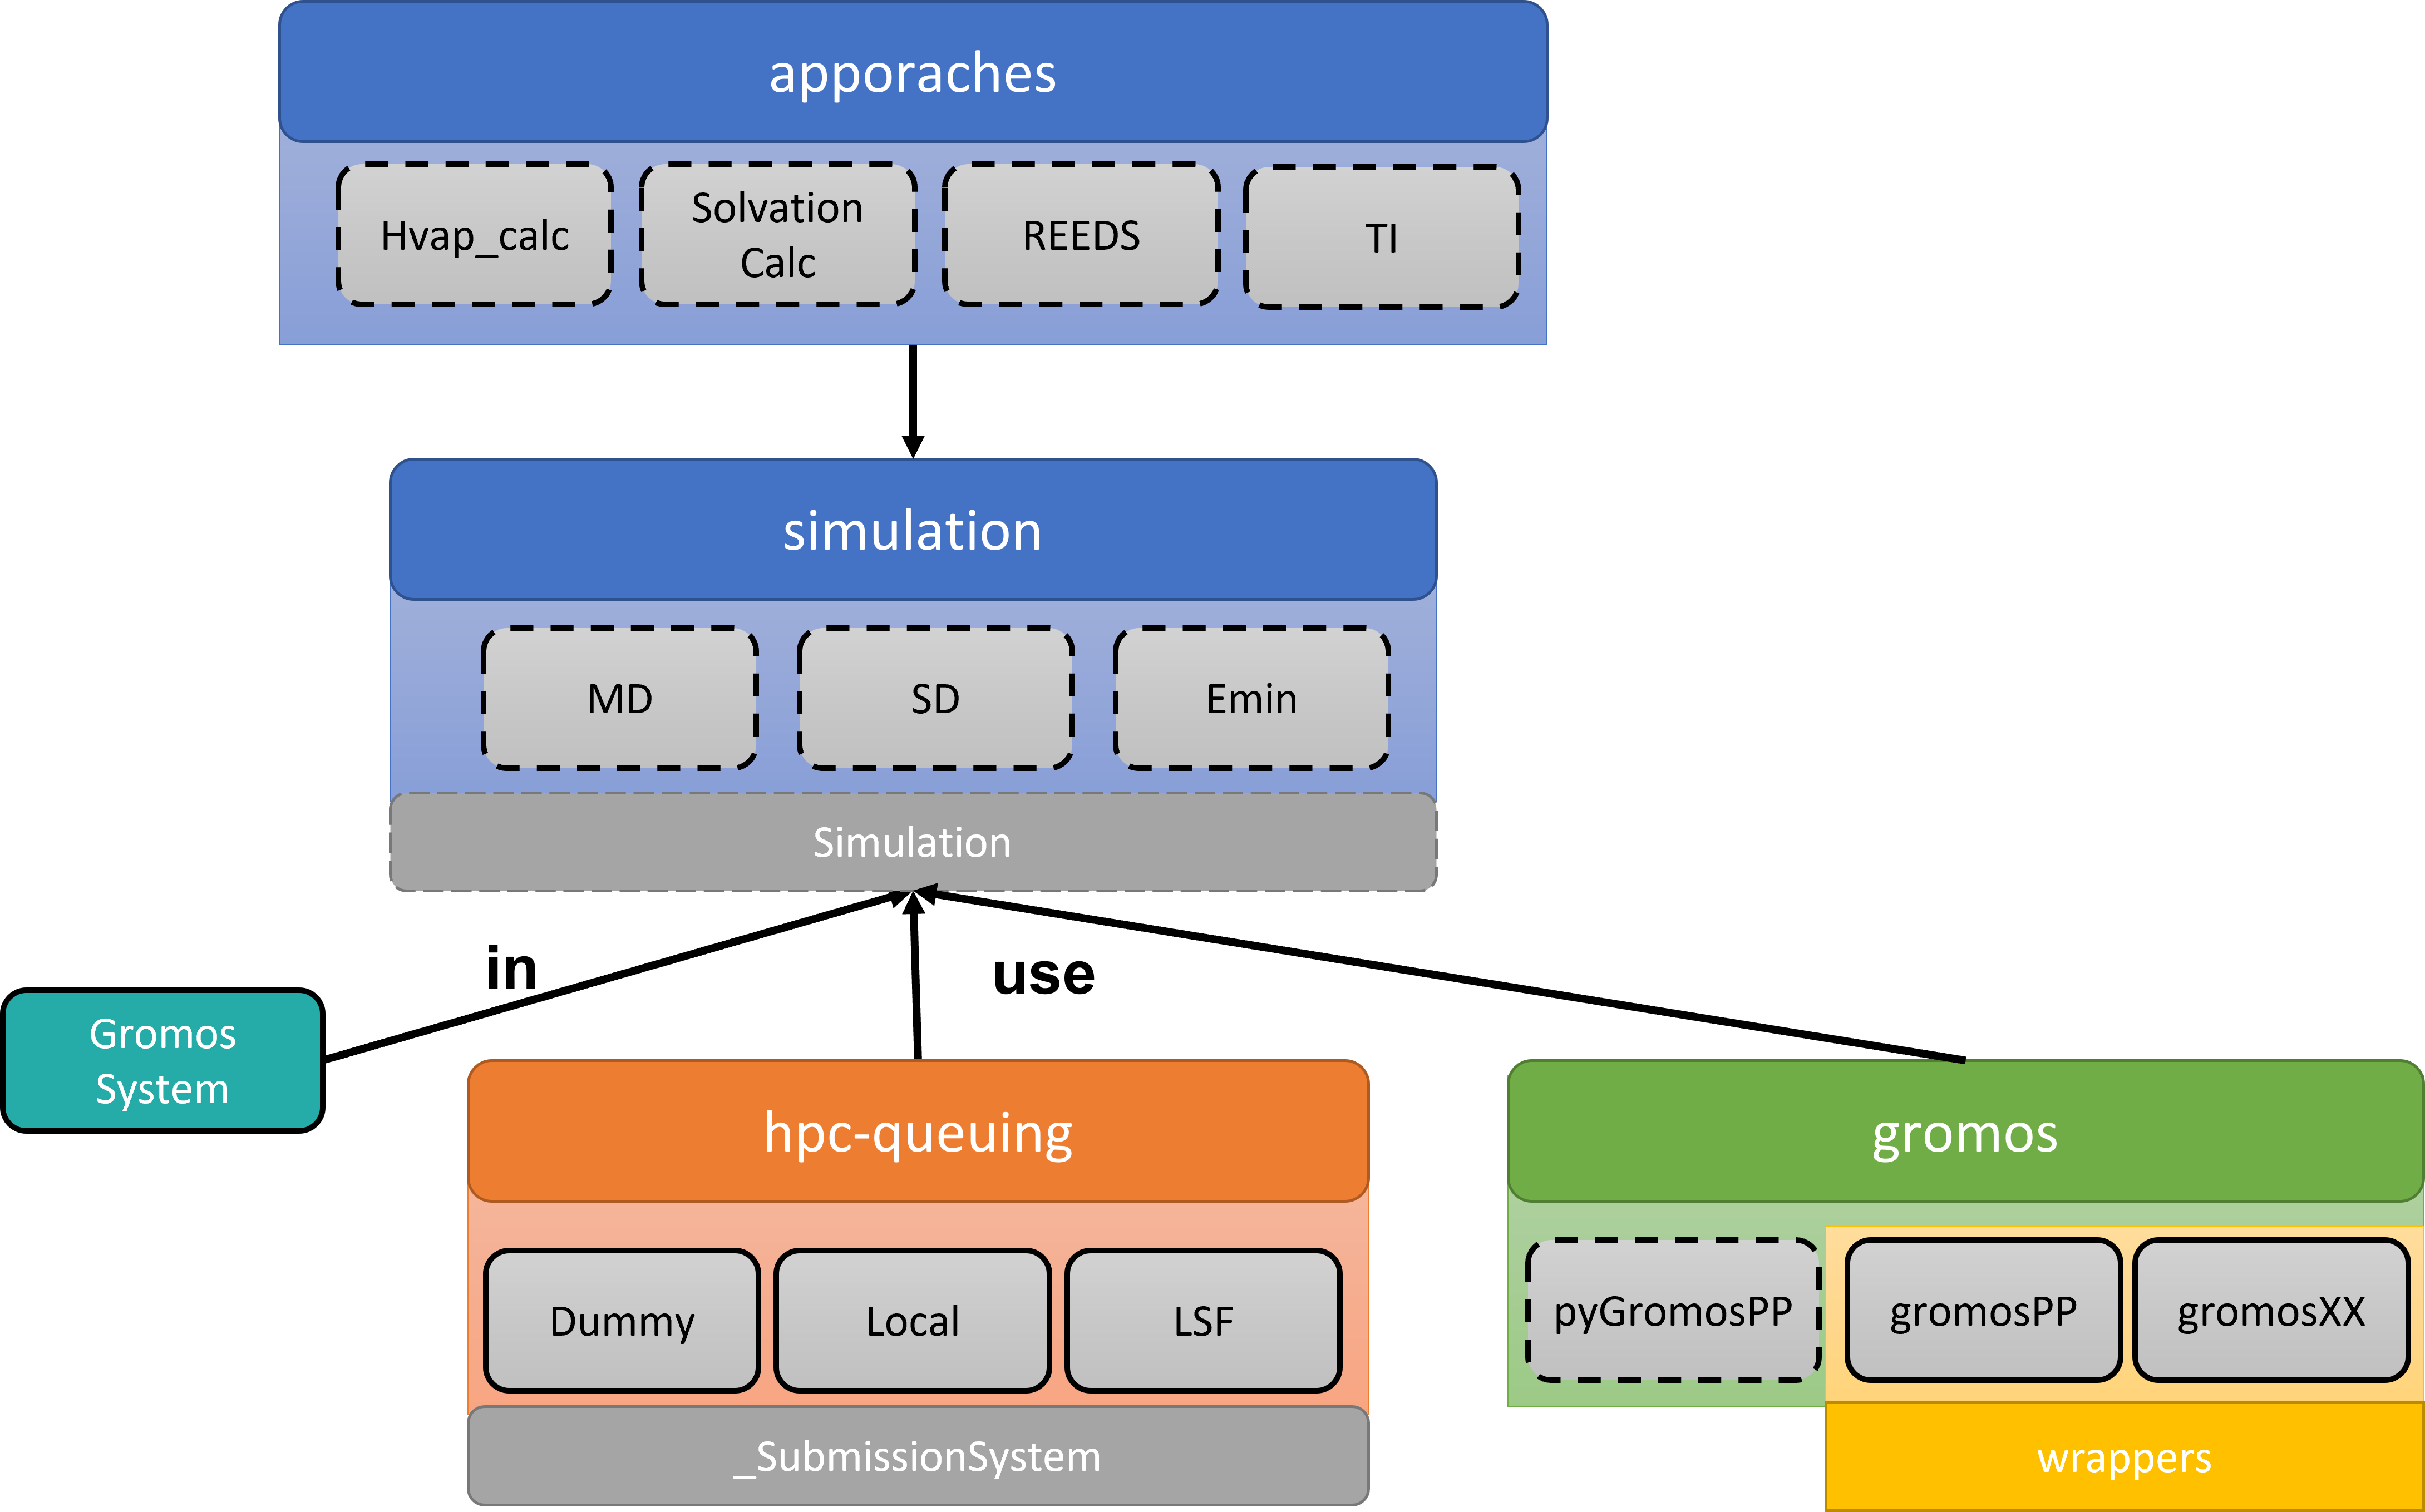
\includegraphics[width=\textwidth]{fig/implementation/Simulation.png}
    \caption{PyGromosTools \textbf{simulations} module contains four submodules, \textbf{hpc-queuing}, \textbf{gromos}, \textbf{simulation}, \textbf{approaches}. \textbf{gromos} is the API to all GROMOS and GROMOS++ functionality written in C++ as well as to a new module containing GROMOS++-like functionality in Python. The \textbf{hpc-queuing} submodule is used to set up simulations in different environments quickly (e.g., local execution or queuing with the LSF job management tool on a cluster). This is possible due to the commonly shared parent class \textit{\_SubmissionSystem}. Dashed lines around boxes represent functions, while bold lines around boxes imply an underlying class structure.}
    \label{fig: SimulationModule}
\end{figure}

The \textbf{hpc-queuing} submodule builds an interface to job management tools like LSF by IBM, and provides the functionality of job queueing for PyGromosTools scripts. The submodule is divided into a submission system and a job scheduling part. The \textbf{submission systems} is structured into an OOP-based structure with the parent class \textit{\_SubmissionSystem} that functions as an interface, ensuring the correct implementation of the child classes. Already implemented classes in \textbf{submission systems} are: 
\begin{itemize}
\item \textit{DUMMY} -- a class meant for testing that only prints out strings. 
\item \textit{LOCAL} -- a class to execute a submitted job directly on the local machine via the operating system.
\item \textit{LSF} -- a class to use the LSF queueing system for scheduling simulations on a HPC cluster. The class is currently optimized for the ETH HPC cluster Euler (\url{https://scicomp.ethz.ch/wiki/Euler}).
\end{itemize}
Besides the submission systems, the \textbf{hpc-queuing} submodule contains job scheduling tools that implement a scheduler-worker pattern (Figure \ref{fig: SimulationExecPattern}). In this pattern, a scheduler function submits worker sub-scripts, which are dynamically generated from template workers, to the queueing system, effectively executing the submitted steps in order. Implemented workers are the simulation, the clean-up, and the analysis worker. The separation of these three tasks is essential to guarantee their correct execution.
%
A good usage of the submission systems is to first develop and debug a pipeline with the DUMMY or LOCAL submission system, and only move to the HPC cluster once the scripts work as intended.

\begin{figure}[h]
    \centering
    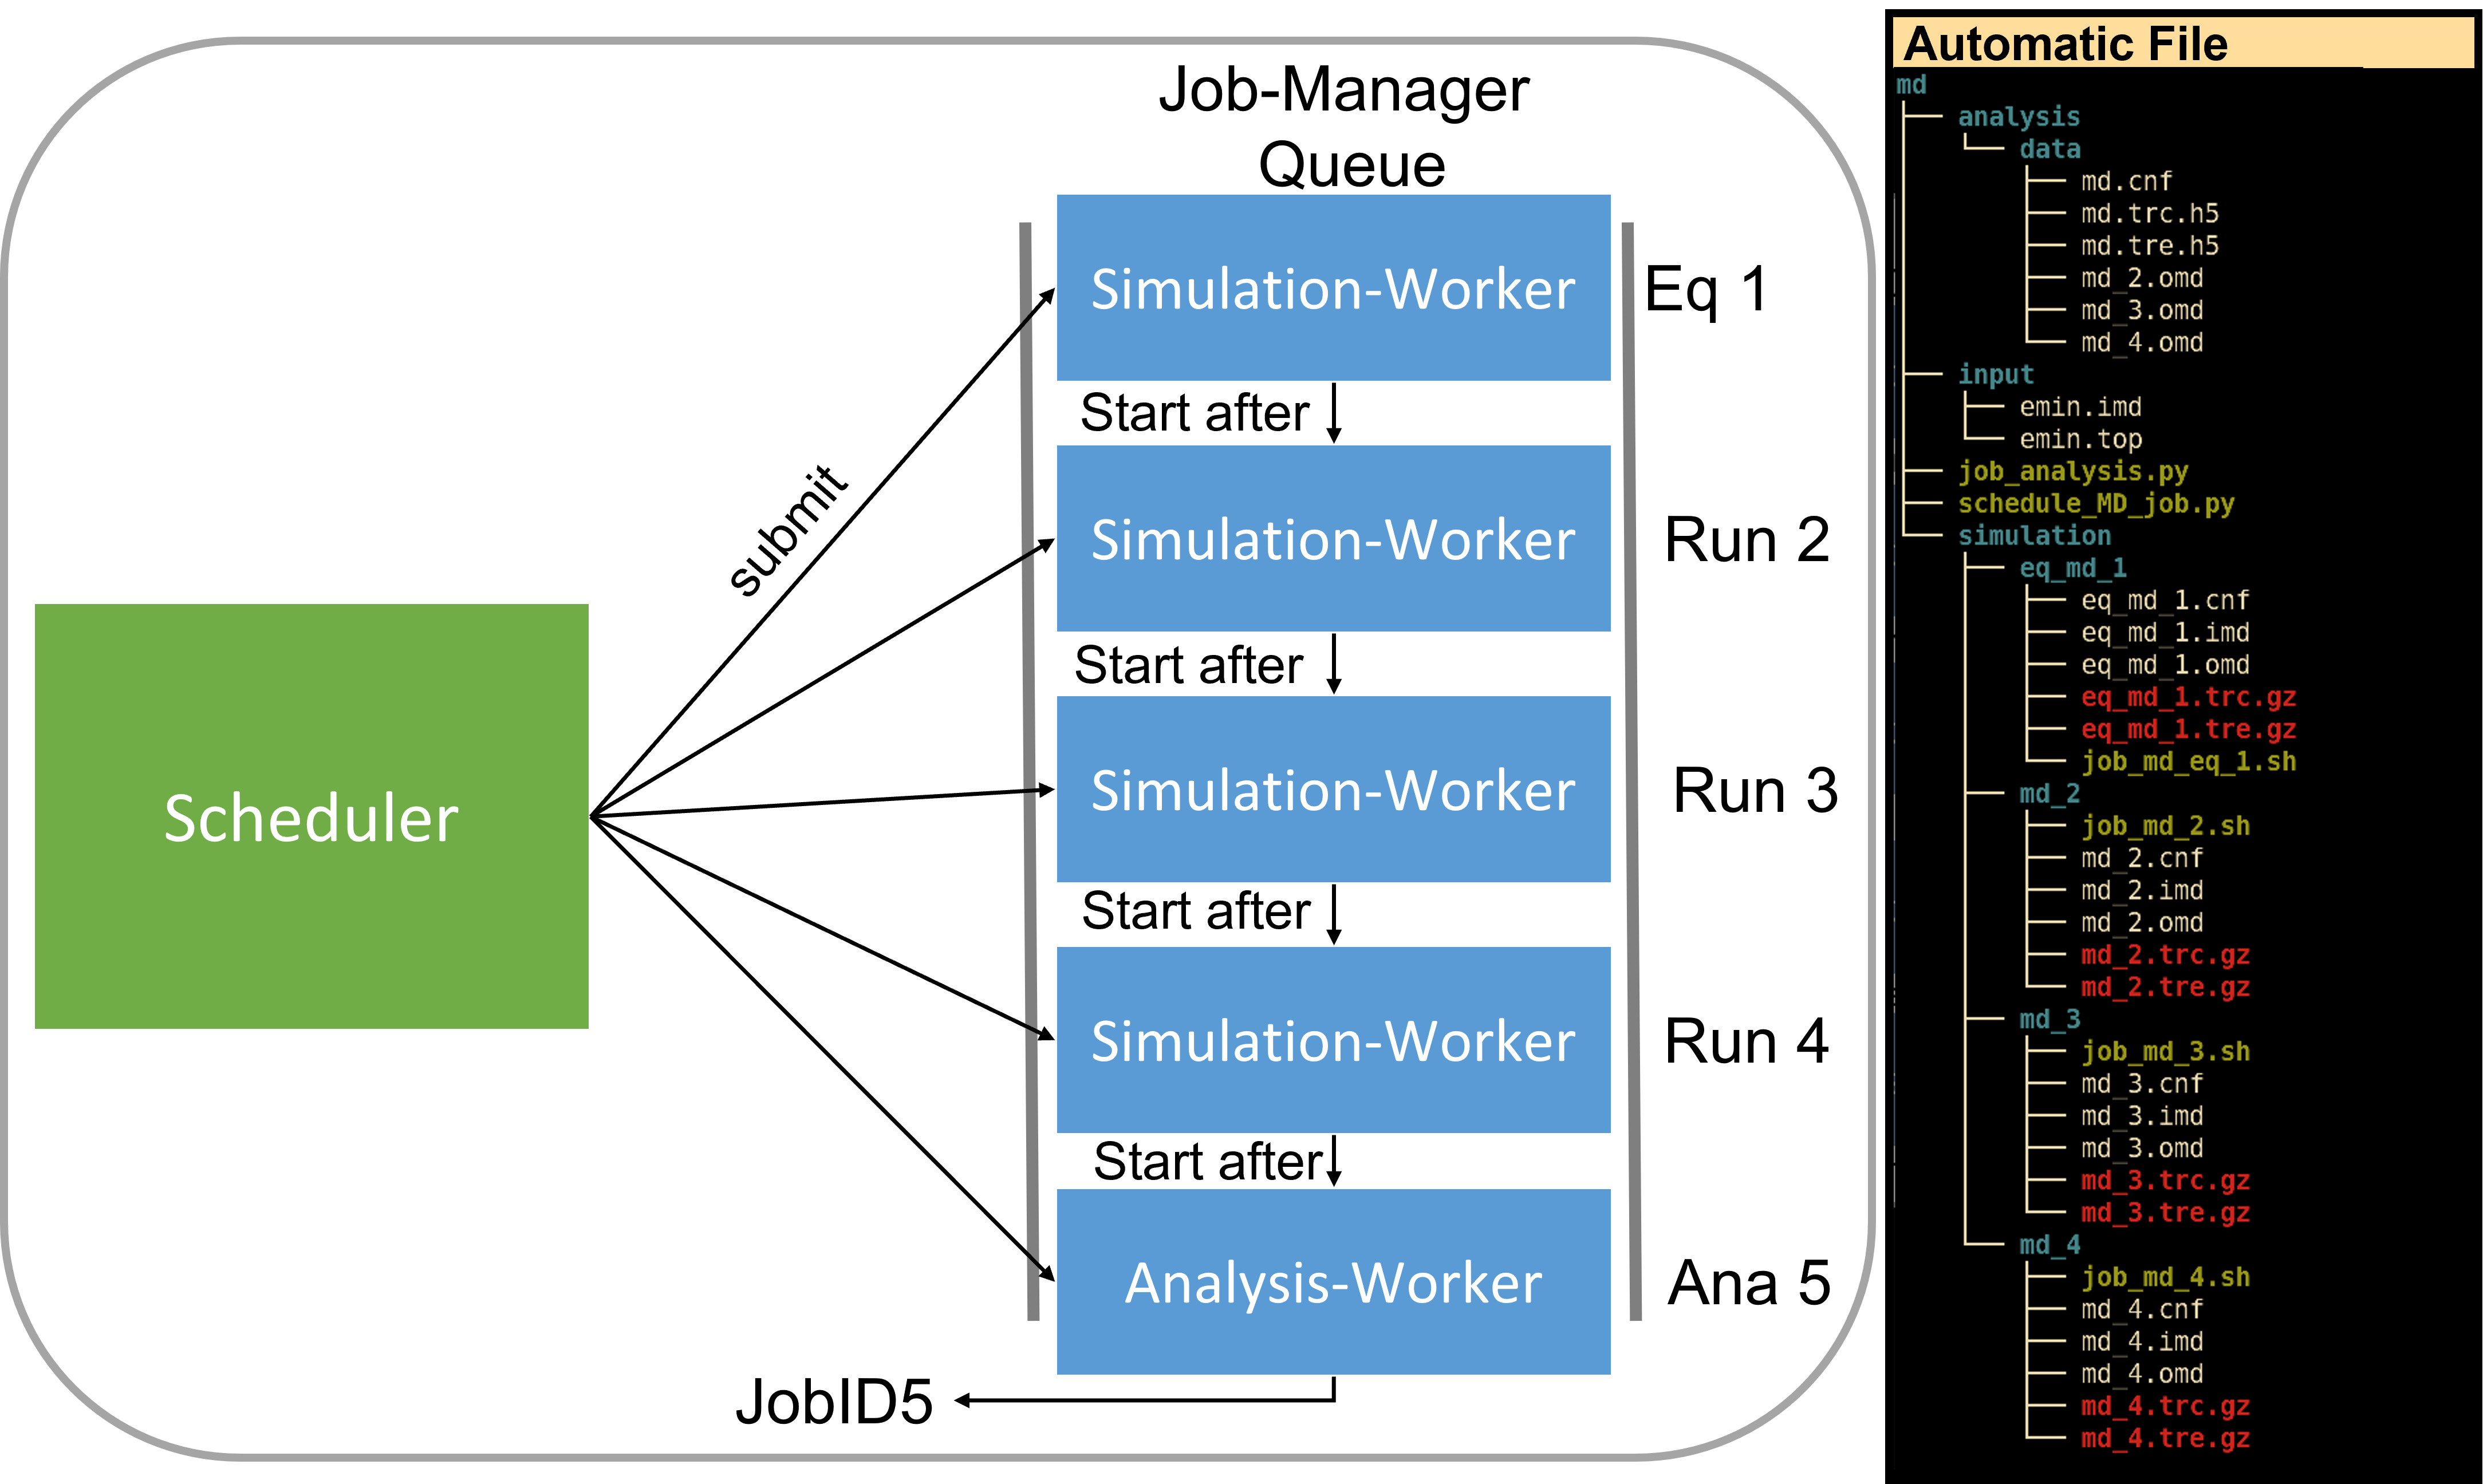
\includegraphics[width=\textwidth]{fig/implementation/SimulationExecutionManagment.png}
    \caption{(Left): HPC-queuing submission pattern using a scheduler function, which submits worker scripts that perform the whole work or a part of it. The worker script is directly executed or submitted to a job management tool based on the provided submission system class. (Right): Automatically generated file structure. Note that the simulation directory is compressed in the process. The md directory is decompressed in the figure to illustrate the concept.
    }
    \label{fig: SimulationExecPattern}
\end{figure}

The two described submodules are combined in the \textit{simulation} function, which executes the simulation. As input, the \textit{simulation} function requires only a \textit{Gromos\_System} with all input files. If no system parameter file (.imd) is provided, a template file for the chosen simulation approach will be mapped onto the system. The default submission system is \textit{LOCAL}, which can be changed to \textit{LSF} for larger jobs. Besides automatic scheduling of tasks, the \textbf{simulation} module also provides automatic file management (Figure \ref{fig: SimulationExecPattern}). The output of the \textit{simulation} function is a copy of the input \textit{Gromos\_System} with the additional output files of the simulation. If the simulation is executed locally, these files are directly parsed into the class. If the simulation is sent to a queue, on the other hand, all not-yet-present output files are marked with a \textit{\_future\_promise} flag. This flag prevents the \textit{Gromos\_System} from executing tasks on the object that requires the presence of the simulation results. In more complex schemes with simulation chaining, these tagged files can be used to submit follow-up simulation steps (e.g., RE-EDS $s$-optimization or energy offset rebalancing\cite{Ries2022}). Once a file is created at a later time point, the \textit{\_future\_promise} flag is removed by the \textit{\_check\_promises} function, and the file is automatically loaded into the \textit{Gromos\_System} object.
Additional smaller features are: checking whether simulations or analysis scripts have finished successfully, checking whether the current job is already submitted to the queue, concatenating files, and storing of trajectories as compressed .h5 files in the analysis/data directory (Figure \ref{fig: SimulationExecPattern}).

The final component of the \textbf{simulations} module is the \textbf{approaches} submodule. In this submodule, top-level simulation approaches are stored, e.g., for calculating solvation free energies, binding free energies, or heats of vaporization. The provided functions offer a high level of automation. For example, the only required input for the calculation of the heat of vaporization is a valid \textit{Gromos\_System} created from a SMILES string. PyGromosTools will automatically create multiple systems (gas phase, liquid phase) and simulations (energy minimization, equilibration, and production run). After all the simulations have been submitted and executed, the analysis will be performed. In this case, the calculated heat of vaporization will be returned for the provided SMILES.


\subsubsection{Analysis and Data Modules}
The \textbf{analysis} module provides functionality for analyzing simulation properties (e.g., atom-positional RMSD, free-energy differences, etc.) and visualizing 3D structures directly in the Jupyter notebook using py3dmol \cite{Rego2014}. Also time series of properties can be visualized using matplotlib \cite{Hunter2007}. The \textbf{analysis} module is the ``youngest'' one in PyGromosTools and will be further extended in the future. 
Finally, the \textbf{data module} provides parameters for the GROMOS 54A7 force field \cite{Schmid2011} together with template simulation parameter files for good starting points.


\FloatBarrier